% !TeX root = ../main.tex

\section{Exercise Questions}

\subsection{Linear Regression}
\subsubsection{Identically distributed and independent}
    A company selling glasses called $TenebrisOttica$ asks us to provide a method to estimate the total amount of sales (in terms of number of glasses sold) at the end of the month. The business unit is expecting to have a daily update of this estimate.\\
    Do you think that it is appropriate to use an ML approach to solve the previous problem? Which assumptions are required to allow the use of ML for the above application?

    \fbox{\begin{minipage}{\linewidth}
        A crucial assumption required for the application of ML is that the samples are i.i.d. In this specific application the data may be temporally dependent and the process generating data may change over time, therefore the data are not independent nor identically distributed.\\
        However, considering a large enough window of data and providing prediction over a time short time period, i.e., so that the nonstationarity is not significant, one might apply ML techniques.
    \end{minipage}}

    Assuming that the above assumptions are satisfied, model the above problem using a Machine Learning approach. Suggest both the data one needs and a proper ML method to solve it.

    \fbox{\begin{minipage}{\linewidth}
        The problem is a regression one, where the input are information about past sales, product details, and user feedbacks and the output is the number of sales at the end of the month. The model should take into account the temporal distance from the current day to the end of the month. A possible method to solve the problem is constituted by Linear Regression or Gaussian Process Regression.
    \end{minipage}}

    Assuming that the above assumption does not hold, what is the problem setting we are in?

    \fbox{\begin{minipage}{\linewidth}
        In the case we cannot rely on the i.i.d. assumption we are in a time series prediction setting. The environment we are considering is either a stochastic nonstationary one or an adversarial one, if we assume that the competitors are significantly affecting the process.
    \end{minipage}}

\subsubsection{Problems recognition}
    \begin{itemize}
        \item \textbf{Regression problem}
        \begin{itemize}
            \item \textbf{Predicting housing prices for real estate}, consider as features the amount of rooms in a house, its distance to the city center, the presence of nearby facilities facilities (primary school, church, underground), age of the building
        \end{itemize}
        \item \textbf{Classification problem}
        \begin{itemize}
            \item \textbf{Identify inside trading among stock market exchange}, in the specific, this problem can be categorized as an anomaly detection one. We can consider as interesting variables the amount of stock actions of a firm exchanged by traders, their affiliation and information
            about their money transaction.
            \item \textbf{Determine which bird species is/are given on audio recording}, in this case, we would need a dataset composed by the couples audio recording/species from all the species we would like to discriminate.
            \item \textbf{Recognise handwritten digits}, if we want to categorize a handwritten digit into the classes 0, . . . , 9 we need images of handwritten digits as features, coupled with the correct class. One might also consider it as a twofold problem of identifying the correct features in an image and then classification into 10 classes.
        \end{itemize}
        \item \textbf{Feature extraction/selection}
        \begin{itemize}
            \item \textbf{Detect interesting features from an image}, one of the most popular approach considered nowadays is the one offered by deep networks which automatically identifies the interesting features from an image for a given task.
        \end{itemize}
        \item \textbf{Dynamic programming}
        \begin{itemize}
            \item \textbf{Pricing goods with stock}, some states (\#goods in my stock)
        \end{itemize}
        \item \textbf{Reinforcement learning}
        \begin{itemize}
            \item \textbf{Teach a robot to play air hockey}, Q-learning or SARSA, as information we consider records from air hockey matches played by humans
            \item \textbf{Maze escape}, repeat same action in different places of maze with different rewards (so no MAB) and we do not know structure of maze (so no DP)
            \item \textbf{Pricing goods with stock}, some states (\#goods in my stock)
        \end{itemize}
        \item \textbf{MAB}
        \begin{itemize}
            \item \textbf{Pricing goods for an e-commerce website}, online learning problem, the problem of pricing a good, in the case we do not have information about the user, is a problem of selecting the best action in the shortest time. Here, we simply need the outcome of newly seen buyers. In the case we have information about users we might resort to techniques
            coming from the recommendation field
            \item \textbf{Pricing goods without stock}, if I sell pencil now or in 3 years same price
            \item \textbf{Optimal bandwidth allocation}, if a lot of users that do not collide stochastic, if hacker adversarial
            \item \textbf{Web ads placement}, assuming pay-per-click scheme and a click event which is stochastic
            \item \textbf{Weather prediction with multiple experts}, expert learning setting, feedback not only of my choice, but also from all possible choice. NO Each time we predict we have rewards coming from all the arms (expert problem). If we use only the feedback coming from the pulled arm, we can use the MAB model, even if we would discard some useful information by doing this
        \end{itemize}
    \end{itemize}

\subsubsection{Input variables}
    Consider a linear regression with input $x$, target $t$ and optimal parameter $\theta^*$.\\
    What happens if we consider as input variables $x$ and $2x$?

    \fbox{\begin{minipage}{\linewidth}
        We are getting a badly conditioned design matrix, as $x$ and $2x$ are linearly dependent, so the matrix will be singular/not invertible
        $$t=w_0+XW=w_0+w_1x+w_22x=w_0+(w_1+2w_2)x$$
    \end{minipage}}

    What we expect on the uncertainty about the parameters we get by considering as input variables $x$ and $2x$?

    \fbox{\begin{minipage}{\linewidth}
        The parameters we get have high variance, since we have an infinite number of couples of parameters minimizing the loss of the samples in the considered problem
        $$t=w_1x+w_22x=(w_1+2w_2)x$$
        Can be satisfied by an infinite number of solutions
    \end{minipage}}

    Provide a technique to solve the problem.

    \fbox{\begin{minipage}{\linewidth}
        Can either
        \begin{itemize}
            \item Remove linearly correlated parameter
            \item Use ridge or lasso and hope at some point one feature will be removed (but if regularization too strong can introduce bias)
        \end{itemize}
    \end{minipage}}

    What happens if we consider as input variables $x$ and $x^2$?
    
    \fbox{\begin{minipage}{\linewidth}
        No linear dependency, no problem
    \end{minipage}}

\subsubsection{Gradient descent}
    Consider an initial parameter $w^{(0)}=[0\,\,0\,\,1]^T$ and a loss function of the form:
    $$J(w)=\frac{1}{2N}\sum_{n=1}^N\left(w^Tx_n-t_n\right)^2$$
    Derive the update given from the gradient descent for the datum $x_1=[1\,\,3\,\,2]^T,\,\,t_1=4$ and a learning rate $\alpha=0.3$

    \fbox{\begin{minipage}{\linewidth}
        For gradient descent:
        $$w^{(k+1)}=w^{(k)}-\alpha^{(k)}\nabla L(x_n)$$
        $$w^{(k+1)}=w^{(k)}-\alpha^{(k)}\left(w^{(k)^T}\phi(x_n)-t_n\right)\phi(x_n)$$
        So:
        $$
        w^{(1)}=w^{(0)}-0.3\left(
            (0\,\,0\,\,1)
            \begin{pmatrix}
                1\\
                3\\
                2
            \end{pmatrix}
            -4
        \right)\begin{pmatrix}
            1\\
            3\\
            2
        \end{pmatrix}
        =\begin{pmatrix}
            0\\
            0\\
            1
        \end{pmatrix}-0.3
        \begin{pmatrix}
            -2\\
            -6\\
            -4
        \end{pmatrix}
        =\begin{pmatrix}
            0.6\\
            1.8\\
            2.2
        \end{pmatrix}
        $$
    \end{minipage}}

    What changes if we want to performa a batch update with $K=10$ data?

    \fbox{\begin{minipage}{\linewidth}
        We can use the batch update formulation
        $$w^{(1)}=w^{(0)}-\frac{\alpha}{K}\sum_{n=1}^K(w^{(0)^T}\phi(x_n)-t_n)\phi(x_n)$$
    \end{minipage}}

\subsubsection{Hypothesis testing}
    We run a linear regression and the slope estimate is $\hat{w}_k=0.5$ with estimated standard error of $\hat{\sigma}v_k=0.2$. What is the largest value of $w$ for which we would NOT reject the null hypothesis that $\hat{w}_1=w$? (hint: assume normal approximation to t distribution, and that we are using the $\alpha=5\%$ significance level for a two-sided test).

    \fbox{\begin{minipage}{\linewidth}
        We know that the variable $S=\frac{\hat{w}_k-w_k}{\hat{\sigma}v_k}$ is distributed as a t-student distribution with $N-M-1$ degree of freedom. If we use the Gaussian approximation we might say that $S\sim\mathcal{N}(0,1)$ To not reject the null hypothesis:
        $$
        \left|\frac{\hat{w}_k-w_k}{\hat{\sigma}v_k}\leq z_{1-\alpha/2}\right|
        $$
        $$
        -z_{1-\alpha/2}\leq\frac{\hat{w}_k-w_k}{\hat{\sigma}v_k}\leq z_{1-\alpha/2}
        $$
        $$
        \hat{w}_k-z_{1-\alpha/2}\hat{\sigma}v_k\leq w_k\leq \hat{w}_k+z_{1-\alpha/2}\hat{\sigma}v_k
        $$
        where we are using the symmetry properties of the Gaussian distribution. We find the maximum value $w_k$ for which we would not reject the null hypothesis:
        $$w_k=\hat{w}_k+z_{1-\alpha/2}=0.5+1.96*0.2$$
    \end{minipage}}

\subsubsection{Least squares and Gaussian Bayesian linear regression}
    Let us assume that the solution with LS method of a regression problem on a specific dataset has as a result:
    $$\hat{t}=5+4x$$
    We would like to repeat the same regression with a Gaussian prior over the parameter space $[w_0,\,\,w_1]$ with mean $\mu=[3,\,\,2]^T$ and covariance matrix $\sigma^2=I_2$ (identity matrix of order 2).\\
    Which one/ones of the following parameters $w$ is/are consistent solution/solutions to the previous regression problem with the previously specified Bayesian prior?
    \begin{enumerate}
        \item $w=[5,\,\,4]$
        \item $w=[4,\,\,3]$
        \item $w=[6,\,\,5]$
        \item $w=[3,\,\,2]$
    \end{enumerate}
    \fbox{\begin{minipage}{\linewidth}
        \begin{itemize}
            \item $P(D|w)=\mathcal{N}(t|\Phi w,\sigma^2I_N)$, likelihood
            \item $P(w)=\mathcal{N}(w|w_0,S_0)$, prior
            \item $P(w|D)=\mathcal{N}(w|w_N,S_N)$, posterior
        \end{itemize}
        Where:
        $$\mathcal{N}(\mu,\sigma^2)=\frac{1}{\sigma\sqrt{2\pi}}e^{-\frac{1}{2}\left(\frac{x-\mu}{\sigma}\right)^2}$$
        $$w_N = S_N(S_0^{-1} w_0 + \frac{\Phi ^T t}{\sigma ^2})$$
        $$S_N ^{-1} = S_0^{-1} + \frac{\Phi ^T \Phi}{\sigma ^2 }$$
        Since here we are considering the Least Square method, the only feasible points for the posterior of the parameter vector are lying on the segment between [5; 4] and [3; 2] (excluding the extreme points which might occur if we have infinite or zero data, respectively).\\
        \textbf{Draw a segment on a $w_0;w_1$ plane, the $w$ inside the segment are consistent}
        \begin{enumerate}
            \item NOT CONSISTENT: Since the prior does not coincide with the MLE solution it is not possible that the solution does not change.
            \item CONSISTENT: The effect of the prior moves the solution towards the areas in the parameter space where the prior has higher probability.
            \item NOT CONSISTENT: The effect of the prior does not allow the solution to move further to the region of prior maximal probability, i.e., the point [3, 2]
            \item NOT CONSISTENT: Since the prior does not coincide with the MLE solution it is not possible that the solution coincides with the prior
        \end{enumerate}
    \end{minipage}}

\subsubsection{K-nearest neighbour for regression}
    Consider a K-NN model for regression and the following training dataset that includes the one-dimensional feature $x$, the target $t$ and the real function $f(x)$ (unknown to the model)
    \begin{tabularx}{\linewidth}{c|X X X X X X}
        \toprule
        \endfirsthead
        \toprule
        \midrule
        \endhead
        \footnotesize [Continues on next page]
        \endfoot
        \bottomrule
        \endlastfoot
        %body
        $x$ & 1 & 1.5 & 3 & 4.5 & 5.5 & 6.5\\
        $t$ & 2.5 & 2.5 & 6 & 10 & 10.5 & 12\\ \midrule
        $f(x)$ & 2 & 3 & 6 & 9 & 11 & 13
    \end{tabularx}
    Compute the predictions for each element in the given dataset obtained by the model with $K=3$

    \fbox{\begin{minipage}{\linewidth}
        According to the K-NN model we compute the predictions as $y(x)=\frac{1}{K}\sum_{i=1}^Kt_i$ where $t_i$ are the targets of the K-NNs (Euclidean distance, include itself in the neighbours)
        \begin{tabularx}{\linewidth}{c|X X X X X X}
            \toprule
            \endfirsthead
            \toprule
            \midrule
            \endhead
            \footnotesize [Continues on next page]
            \endfoot
            \bottomrule
            \endlastfoot
            %body
            $x$ & 1 & 1.5 & 3 & 4.5 & 5.5 & 6.5\\ \midrule
            $y(x)$
            & $\frac{2.5+2.5+6}{3}=\frac{11}{3}$
            & $\frac{2.5+2.5+6}{3}=\frac{11}{3}$
            & $\frac{2.5+6+10}{3}=\frac{37}{6}$
            & $\frac{6+10+10.5}{3}=\frac{53}{6}$
            & $\frac{10+10.5+12}{3}=\frac{65}{6}$
            & $\frac{10+10.5+12}{3}=\frac{65}{6}$\\ \midrule
        \end{tabularx}
    \end{minipage}}

    Compute the mean squared error on the given dataset

    \fbox{\begin{minipage}{\linewidth}
        Use
        $$\frac{1}{N}\sum_{i=1}^N(t_i-y(x_i))^2=\frac{
            \left(\frac{11}{2}-2.5\right)^2+
            \left(\frac{11}{2}-2.5\right)^2+
            \left(\frac{37}{6}-6\right)^2+
            \left(\frac{53}{6}-10\right)^2+
            \left(\frac{65}{6}-10.5\right)^2+
            \left(\frac{65}{6}-12\right)^2
        }{6}$$
    \end{minipage}}

    Provide an estimate of the variance of the model with the available data. What happens to the variance if we increase $K$?

    \fbox{\begin{minipage}{\linewidth}
        Use:
        $$\frac{\hat{Var}[t]}{K}=\frac{
            \frac{1}{N}\sum_{i=1}^N(t_i-f(x_i))^2
        }{K}$$
        $$
        =\frac{
            (2.5-2)^2+
            (2.5-3)^2+
            (6-6)^2+
            (10-9)^2+
            (10.5-11)^2+
            (12-13)^2
        }{6K}
        $$
        Thus increasing $K$ would make the variance smaller
    \end{minipage}}

    Provide an estimate of the squared bias of the model with the available data. What happens to the bias if we increase $K$?

    \fbox{\begin{minipage}{\linewidth}
        Use:
        $$\frac{1}{N}\sum_{i=1}^N(f(x_i)-y(x_i))^2$$
        $$
        =\frac{
            (\frac{11}{3}-2)^2+
            (\frac{11}{3}-3)^2+
            (\frac{37}{6}-6)^2+
            (\frac{53}{6}-9)^2+
            (\frac{65}{6}-11)^2+
            (\frac{65}{6}-13)^2
        }{6}
        $$
        While $K$ does not explicitly appears in the formula, it affects the $y(x)$ values, and we can expect the bias to increase if we increase $K$
    \end{minipage}}

\subsection{Linear Classification}
\subsubsection{Perceptron}
    Consider a binary perceptron classifier defined by the parameters $w=[2,\,\,1,\,\,1]^T$ with features vector $\phi([a,b])=[a,\,\,b,\,\,ab]^T$.\\
    Given a new data point $(x,t)=([a,b],t)$, explain the procedure you would follow to decide whether the classifier should be retrained.

    \fbox{\begin{minipage}{\linewidth}
        First, we should check if the new data point is correctly classified, i.e., whether
        $$sign(w^T\phi(x))=sign([2,1,1]*[a,b,ab]^T)=t$$
        If the answer is positive we do not retrain, otherwise retrain, i.e. using stochastic gradient descent method until convergence
    \end{minipage}}

    Consider the data point $(x_1,t)=([-1,-2],+1)$. Update the classifier with the perceptron algorithm ($\alpha=1$)

    \fbox{\begin{minipage}{\linewidth}
        $$sign(w^T\phi(x))=sign([2,1,1]*[-1,-2,2]^T)=sign(-2)=-1$$
        The point is missclassified, so we have to update the model using:
        $$w^{(k+1)}=w^{(k)}-\alpha\nabla L_P(w)=w^{(k)}+\alpha\phi(x_n)t_n$$
        $$
        w=\begin{pmatrix}
            2\\
            1\\
            1         
        \end{pmatrix}+1*
        \begin{pmatrix}
            -1\\
            -2\\
            2
        \end{pmatrix}*1=
        \begin{pmatrix}
            1\\
            -1\\
            3
        \end{pmatrix}
        $$
    \end{minipage}}

    After the previous updates to the classifier, can we say the retrain procedure is completed?

    \fbox{\begin{minipage}{\linewidth}
        No, since we have updated the classifier, we should check if all the other data points in the dataset are still correctly classified
    \end{minipage}}

\subsubsection{Perceptron confusion matrix}
    Consider a binary classifier trained on a dataset made of $N=100$ samples.\\
    Suppose that the $Precision=0.25,\,\,F1=0.4$, compute the Recall.

    \fbox{\begin{minipage}{\linewidth}
        Reminder
        \begin{itemize}
            \item \textbf{Accuracy}, proportion of points classified/all points
            $$Acc=\frac{t_p+t_n}{N}$$
            \item \textbf{Precision}, amount of \textbf{true positives} with respect to the total amount of points classified as positive: how many selected items are relevant?
            $$Pre=\frac{t_p}{t_p+f_p}$$
            \item \textbf{Recall}, how many points in positive class are correctly classified? How many relevant items are selected?
            $$Rec=\frac{t_p}{t_p+f_n}$$
            \item \textbf{F1 score}, close to 1 good, close to 0 poor classifier
            $$F1=2\,\frac{Pre*Rec}{Pre+Rec}$$
        \end{itemize}
        So:

        \vspace{1em}
        $
        F1*Rec+F1*Pre=2Pre*Rec
        \\\cdots=F1*Pre=2Pre*Rec-F1*Rec
        \\\cdots=Rec=\frac{F1*Pre}{2Pre-F1}=1
        $
    \end{minipage}}

    Knowing in addition that $Accuracy=0.85$, compute the full confusion matrix

    \fbox{\begin{minipage}{\linewidth}
        As $N=100$
        $$
        \begin{cases}
            Acc=0.85=\frac{t_p+t_n}{100}\\
            Pre=0.25=\frac{t_p}{t_p+f_p}\\
            Rec=1=\frac{t_p}{t_p+f_n}\\
            t_p+t_n+f_p+f_n=100
        \end{cases}
        \Rightarrow
        \begin{cases}
            85=t_p+t_n\\
            f_p=3t_p\\
            f_n=0\\
            t_p+t_n+f_p+f_n=100
        \end{cases}
        \Rightarrow
        \begin{cases}
            t_p=5\\
            t_n=80\\
            f_p=15\\
            f_n=0
        \end{cases}
        $$
        \begin{tabularx}{\linewidth}{X|X|X}
            \toprule
            \textbf{} & \textbf{Actual Class: 1} & \textbf{Actual Class: 0}\\
            \midrule
            \endfirsthead
            \toprule
            \textbf{} & \textbf{Actual Class: 1} & \textbf{Actual Class: 0}\\
            \midrule
            \endhead
            \footnotesize [Continues on next page]
            \endfoot
            \bottomrule
            \endlastfoot
            %body
            \textbf{Predicted Class: 1} & $t_p=5$ & $f_p=15$\\ \midrule
            \textbf{Predicted Class: 0} & $f_n=0$ & $t_n=80$\\ \midrule
        \end{tabularx}
    \end{minipage}}

    In which circumstances the Accuracy is not a reliable index to assess the quality of trained model?

    \fbox{\begin{minipage}{\linewidth}
        Not reliable when:
        \begin{itemize}
            \item Data is unbalanced
            \item When the importance of wrongly predicting positive-class sampels is different from wrongly predicting negative-class samples
        \end{itemize}
    \end{minipage}}

\subsubsection{Logistic regression}
    Suppose we collect data for a group of workers with variables hours spent working $x_1$, number of completed projects $x_2$ and receive a bonus $t$. We fit a logistic regression and produce estimated coefficients: $w_0=-6,\,\,w_1=0.05,\,\,w_2=1$.\\
    Estimate the probability that a worker who worked for 40h and completed 3.5 projects gets a bonus.

    \fbox{\begin{minipage}{\linewidth}
        The two classes are getting a bonus ($C_1$) and not getting one
        $$p(C_1|\phi)=\frac{1}{1+exp(-w^T\phi)}=\sigma(w^T\phi)$$
        The denominator is:
        $$
        1+exp\left(
            -(-6\,\,\,0.05\,\,\,1)\begin{pmatrix}
                1\\
                40\\
                3.5
            \end{pmatrix}
        \right)=1+exp(0.5)
        $$
        So
        $$p(C_1|\phi)=\frac{1}{1+exp(0.5)}=0.3775$$
    \end{minipage}}

    How many hours would that worker need to spend working to have a 50\% chance of getting a bonus?

    \fbox{\begin{minipage}{\linewidth}
        $$
        \frac{1}{2}=\frac{1}{1+exp(-w^t\phi)}
        \Rightarrow e^{-w^T\phi}=1\Rightarrow-w^T\phi=0
        $$
        $$
        (-6\,\,\,0.05\,\,\,1)\begin{pmatrix}
                1\\
                \hat{x_1}\\
                3.5
            \end{pmatrix}
        =0\Rightarrow \hat{x_1}=\frac{2.5}{0.05}=50
        $$
    \end{minipage}}

    Do you think values of $z$ in $\sigma(z)$ lower than -6 make sense in this problem?

    \fbox{\begin{minipage}{\linewidth}
        Since all the considered variables are positive definite, it makes only sense to consider values greater than -6 as predictions
    \end{minipage}}

\subsubsection{Naive Bayes}
    Consider the following dataset to implement a spam filter function
    \begin{tabularx}{\linewidth}{X|X|X|X|X|X}
        \toprule
        \textbf{pills} & \textbf{fee} & \textbf{kittens} & \textbf{URL presence} & \textbf{PoliMi} & \textbf{spam}\\
        \midrule
        \endfirsthead
        \toprule
        \textbf{pills} & \textbf{fee} & \textbf{kittens} & \textbf{URL presence} & \textbf{PoliMi} & \textbf{spam}\\
        \midrule
        \endhead
        \footnotesize [Continues on next page]
        \endfoot
        \bottomrule
        \endlastfoot
        %body
        0 & 1 & 0 & 0 & 1 & 0\\
        0 & 0 & 1 & 1 & 0 & 0\\
        0 & 0 & 1 & 0 & 0 & 0\\
        0 & 0 & 1 & 0 & 1 & 0\\
        0 & 0 & 0 & 0 & 0 & 0\\ \midrule
        1 & 1 & 0 & 0 & 1 & 1\\
        0 & 1 & 0 & 1 & 0 & 1\\
        1 & 0 & 0 & 1 & 0 & 1
    \end{tabularx}
    Where we enumerate the presence of specific word of an URL in 8 different e-mails and the corresponding inclusion in the spam or non-spam class.\\
    Estimate a Naive Bayes classifier choosing the proper distributions for the classes prior and the feature posteriors.

    \fbox{\begin{minipage}{\linewidth}
        $C_0$= negative class (spam=0)\\
        $C_1$= positive class (spam=1)

        \vspace{1em}
        The proper models in this case uses Bernoulli variables both as prior distributions and for the posteriors. More specifically we estimate the probabilities with the MLE (maximum likelihood estimation), which is the common empirical expected value.\\
        We look at the right-most column which tells us if spam or not, we see 5 of them are not spams (in $C_0$) and 3 of them are spams (in $C_1$)
        $$\hat{p}(C_0)=\frac{5}{8}\hspace{5em}\hat{p}(C_1)=\frac{3}{8}$$
        We denote $p(x_i=\{0,1\}|C_j)$ the probability that feature $i$ equals 0 or 1 considering class $C_j$ (e.g. feature 1 is pills), Bernoulli
        $$p(x_1=1|C_0)=\frac{0}{5}\hspace{5em}p(x_1=1|C_1)=\frac{2}{3}$$
        $$p(x_2=1|C_0)=\frac{1}{5}\hspace{5em}p(x_2=1|C_1)=\frac{2}{3}$$
        $$p(x_3=1|C_0)=\frac{3}{5}\hspace{5em}p(x_3=1|C_1)=\frac{0}{3}$$
        $$p(x_4=1|C_0)=\frac{1}{5}\hspace{5em}p(x_4=1|C_1)=\frac{2}{3}$$
        $$p(x_5=1|C_0)=\frac{2}{5}\hspace{5em}p(x_5=1|C_1)=\frac{1}{3}$$
        For the probabilities of the opposite class just use
        $$p(x_i=\{0,1\}|C_1)=1-p(x_i=\{0,1\}|C_0)$$
    \end{minipage}}

    Predict the probability of the following samples to belong to the spam and no-spam classes
    \begin{tabularx}{\linewidth}{X|X|X|X|X|X}
        \toprule
        \textbf{pills} & \textbf{fee} & \textbf{kittens} & \textbf{URL presence} & \textbf{PoliMi} & \textbf{spam}\\
        \midrule
        \endfirsthead
        \toprule
        \textbf{pills} & \textbf{fee} & \textbf{kittens} & \textbf{URL presence} & \textbf{PoliMi} & \textbf{spam}\\
        \midrule
        \endhead
        \footnotesize [Continues on next page]
        \endfoot
        \bottomrule
        \endlastfoot
        %body
        1 & 1 & 0 & 1 & 0 & ?\\
        0 & 1 & 1 & 0 & 1 & ?
    \end{tabularx}
    \fbox{\begin{minipage}{\linewidth}
        We use
        $$p(C_k|x)=\frac{p(C_k)p(x|C_k)}{p(x)}=\cdots=p(C_k)\prod_{j=1}^Mp(x_j|C_k)$$
        \begin{itemize}
            \item First sample (1 1 0 1 0), we see if it belongs to $C_0$ or not:
            
            \vspace{1em}
            $
            p(C_0|x)=p(C_0)p(x_1=1|C_0)p(x_2=1|C_0)p(x_3=0|C_0)p(x_4=1|C_0)p(x_5=0|C_0)
            \\\cdots=\frac{5}{8}*0*\frac{1}{5}\cdots=0
            $

            \vspace{1em}
            So the point must belong to $C_1$
            \item Second sample (0 1 1 0 1), we see if it belongs to $C_0$ or not:
            
            \vspace{1em}
            $
            p(C_0|x)=p(C_0)p(x_1=0|C_0)p(x_2=1|C_0)p(x_3=1|C_0)p(x_4=0|C_0)p(x_5=1|C_0)
            \\\cdots=\frac{5}{8}*1*\frac{1}{5}*\frac{3}{5}*\frac{4}{5}*\frac{2}{5}=0.024
            $

            \vspace{1em}
            We see if it belongs to $C_1$ or not:

            \vspace{1em}
            $
            p(C_1|x)=p(C_1)p(x_1=0|C_1)p(x_2=1|C_1)p(x_3=1|C_1)p(x_4=0|C_1)p(x_5=1|C_1)
            \\\cdots=\frac{3}{8}*\frac{1}{3}*\frac{2}{3}*0*\cdots=0
            $

            \vspace{1em}
            So the point must belong to $C_0$
        \end{itemize}
    \end{minipage}}

\subsection{Bias-Variance Tradeoff}
\subsubsection{F-statistics for model selection}
    Assume to have two different linear models working on the same dataset of $N=100$ samples
    \begin{itemize}
        \item The first model has $k_1=2$ input, considers linear features and has a residual sum of squares $RSS_1=0.5$ on a validation set
        \item The second model has $k_2=8$ input, considers only quadratic features and has $RSS_2=0.3$ on a validation set
    \end{itemize}
    Which one would you choose? Recall the F-test for statistics for distinguishing between linear models is:
    $$\hat{F}=\frac{N-p_2}{p_2-p_1}\frac{RSS_1-RSS_2}{RSS_2}\sim F(p_2-p_1,N-p_2)$$
    Where $p_1$ and $p_2$ are the two parameters of the two models and $F(a,b)$ is the Fisher distribution with $a$ and $b$ degrees of freedom.\\
    It considers the following hypothesis test:
    $$H_0: w_1 = \dots = w_M = 0 \text{ vs. }  H_1: \exists w_j \neq 0$$
    The F-statistic can be computed and is distributed as follows:
    $$F = \frac{dfe}{M - 1}\frac{\sum_n (\hat{t}_n-t_n)- RSS}{RSS} \sim F_{M-1, N-M} $$
    where $F_{M-1, N-M}$ is the Fisher-Snedecor distribution with parameters $M-1$ and $N-M$

    \fbox{\begin{minipage}{\linewidth}
        The first model has $p_1=k_1+1=3$ parameters\\
        The second one $p_2=k_2+\begin{pmatrix}
            k_2\\
            2
        \end{pmatrix}+1=\underset{Linear\,\,parameters}{\underbrace{k_2}}+\underset{Quadratic\,\,parameters}{\underbrace{\frac{k_2(k_2-1)}{2}}}+1=8+28+1=37$ parameters.\\
        To evaluate if two regressive models, under the assumption that the noise is i.i.d. zero mean Gaussian random variable, we can use an F-test. In the specific, we know that the test statistic is distributed as an F distribution, with $(p_2-p_1,N-p_2)$ degrees of freedom. Thus, we can evaluate the p-value of the statistic $\hat{F}$ computed on the two aforementioned models:
        $$\hat{F}=\frac{100-37}{37-3}\frac{0.5-0.3}{0.3}=1.2353$$
        whose p-value is 0.2311. Thus there is no statistical evidence at confidence level lower than $\alpha$=0.2311 that the second model is better than the first one
    \end{minipage}}

    Consider that the 99th quantile of the Fisher distribution is $F_{99}(100-37,37-3)=F_{99}(63,34) << \hat{F}$, what can you infer?

    \fbox{\begin{minipage}{\linewidth}
        If this is the case, it means that there is statistical evidence at level at least 0.99 that the second model is better than the first one
    \end{minipage}}

\subsubsection{PCA from image}
    \begin{figure}[!ht]
        \begin{minipage}{\linewidth}
            \centering
            \makebox[\textwidth][c]{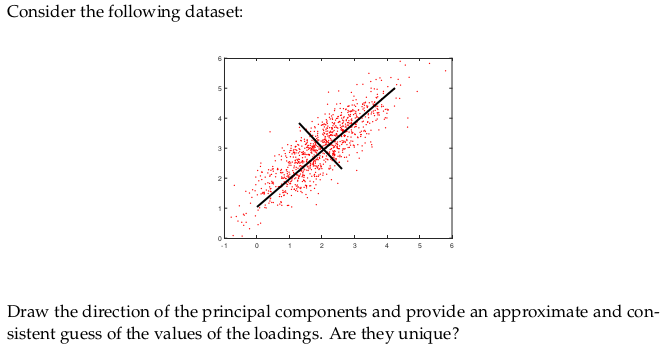
\includegraphics[width=1\textwidth]{images/Bias-Variance Tradeoff_01.png}}%
            %\caption{Nielsen's heuristics evaluation summary}
            %\label{BarsNielsenCrop}
        \end{minipage}
    \end{figure}
    \fbox{\begin{minipage}{\linewidth}
        Let's try to give some numbers to these PCs.\\
        $(0.5\,\,0.5)^T$, is this an eigenvector? No, an eigenvector has norm=1, here $\sqrt{0.5^2+0.5^2}=\sqrt{0.5}$\\
        As first PC is 45°/$\frac{\pi}{4}$:
        $$(\frac{\sqrt{2}}{2}\hspace{0.5em}-\frac{\sqrt{2}}{2})$$
        $$(\frac{\sqrt{2}}{2}\hspace{1.5em}\frac{\sqrt{2}}{2})$$
        They are orthogonal and have norm=1, properties for being PCs. They are not unique, just play with the signs, same direction, different verse
    \end{minipage}}

\subsubsection{PCA loadings}
    You are analysing a dataset where each observation is an age, height, length and width of a turtle. You want to know if the data can be well described by fewer than four dimensions, so you decide to do PCA. Which of the following is most likely to be the loadings of the first PC?
    \begin{enumerate}
        \item $(1,1,1,1)$
        \item $(0.5,0.5,0.5,0.5)$
        \item $(0.71,-0.71,0,0)$
        \item $(1,-1,-1,-1)$
    \end{enumerate}
    \fbox{\begin{minipage}{\linewidth}
        We check the norm: the options 1 and 4 have norms that exceed 1. The most likely correct one is the 2 as we expect this particular set of four variables to be positively correlated with each other in the first PC
    \end{minipage}}

\subsubsection{K-nearest neighbour for classification}
    A KNN classifier classifies a new data point by applying a mojirty voting among its K-nearest neighbour. There are the available data points in the dataset:

    \vspace{1em}
    $
    x_0=(-2,-3,0),\,y_0=1   \hspace{6em}    x_1=(-2,2,-1),\,y_1=1\\
    x_2 = (-2, -1, -3),\,y_2 = 1   \hspace{6em}    x_3 = (2, 1, -4),\,y_3 = 1\\
    x_4 = (2, -3, 2),\,y_4 = 1   \hspace{6em}    x_5 = (1, 2, 2),\,y_5 = 0\\
    x_6 = (-1, 1, -2),\,y_6 = 0   \hspace{6em}    x_7 = (-1, 2, 2),\,y_7 = 1\\
    x_8 = (1, -2, 0),\,y_8 = 0   \hspace{6em}    x_9 = (-3, -3, -2),\,y_9 = 1
    $

    \vspace{1em}
    Classify the new point $x=(0,0,-1)$ according to a KNN classifier trained on the dataset reported, assuming a $K=3$ and using the Euclidean distance

    \fbox{\begin{minipage}{\linewidth}
        We compare all Euclidean distances

        \vspace{1em}
        $
        d(x,x_0)=\sqrt{(0-(-2))^2+(0-(-3))^2+(-1-0)^2}=\sqrt{4+9+1}=\sqrt{14}=3.74\\
        d(x,x_1)=\sqrt{12}=3.46\\
        d(x,x_2)=\sqrt{9}=3\\
        d(x,x_3)=\sqrt{14}=3.74\\
        d(x,x_4)=\sqrt{22}=4.69\\
        d(x,x_5)=\sqrt{14}=3.74\\
        d(x,x_6)=\sqrt{3}=1.73\\
        d(x,x_7)=\sqrt{14}=3.74\\
        d(x,x_8)=\sqrt{6}=2.45\\
        d(x,x_9)=\sqrt{19}=4.36
        $

        \vspace{1em}
        The closest $K=3$ points are $(x_6,x_8,x_2)$, we perform a majority voting within $(y_6,y_8,y_2)=(0,0,1)$, which classifies the new point as 0
    \end{minipage}}

    What happens if $K=10$ instead? Is it a good idea?

    \fbox{\begin{minipage}{\linewidth}
        Since in this case |dataset|=10, if we have more 1's we will always predict 1, if more 0's always zero, so it is a bad idea, always selecting the same class for any point.\\
        Also for good practice we should select an odd value for $K$ in order to avoid ties when doing majority voting
    \end{minipage}}

\subsection{PAC-Learning and VC Dimension}
\subsubsection{VC dimension}
    Show that the VC dimension af an axis aligned rectangle is 4.

    \fbox{\begin{minipage}{\linewidth}
        Two steps:
        \begin{enumerate}
            \item Player 1 chooses $n$ points
            \item Player 2 opponent has to label the points, labelling done in order to let the first player to classify points
        \end{enumerate}
        If player 1 wins, VC dimension at least $n$, else we cannot say anything.\\
        In order to prove VC is a specific number, player 1 must win, otherwise we must show that all possible combinations of points in the space won't let player 1 win: \textbf{check true show one, check false show all}. We want to show
        $$
        VC(C)=4\Rightarrow
        \begin{cases}
            VC(C)\geq 4\\
            VC(C)< 5
        \end{cases}
        $$
        \begin{itemize}
            \item $\mathbf{VC(C)\geq 4}$, P1 chooses $n=4$ points (notice he should not choose align points, otherwise impossible for some combinations), then P2 labels them, for example\\
            \begin{center}
                
\includegraphics[width=0.3\textwidth]{images/Bias-Variance Tradeoff_02.png}           
            \end{center}
            In this way we can always separate with a rectangle, P1 always wins (he was smart by choosing non aligned points).\\
            It is possible to show by enumeration that all possible labelling are shattered by the rectangle
            \item $\mathbf{VC(C) < 5}$, consider 5 points and the set of points with maximum and minimum $x$ coordinate and maximum and minimum $y$ coordinates (the ones that make a perimeter): P2 can now label the one inside the perimeter with - and the ones on the perimeter with +, making the shattering impossible. This is true even if two aligned\\
            \begin{center}
                
\includegraphics[width=0.3\textwidth]{images/Bias-Variance Tradeoff_03.png}
                \hspace{1em}
                
\includegraphics[width=0.3\textwidth]{images/Bias-Variance Tradeoff_04.png}
            \end{center}
        \end{itemize}
    \end{minipage}}\

    Show that the VC dimension of a linear classifier in 2D is 3.

    \fbox{\begin{minipage}{\linewidth}
        $$
        VC(C)=3\Rightarrow
        \begin{cases}
            VC(C)\geq 3\\
            VC(C)< 4
        \end{cases}
        $$
        \begin{itemize}
            \item $\mathbf{VC(C)\geq 3}$, by considering a set of 3 non-aligned points, it is possible to show by enumeration that it is possible to shatter them with a linear classifier:
            \begin{center}
                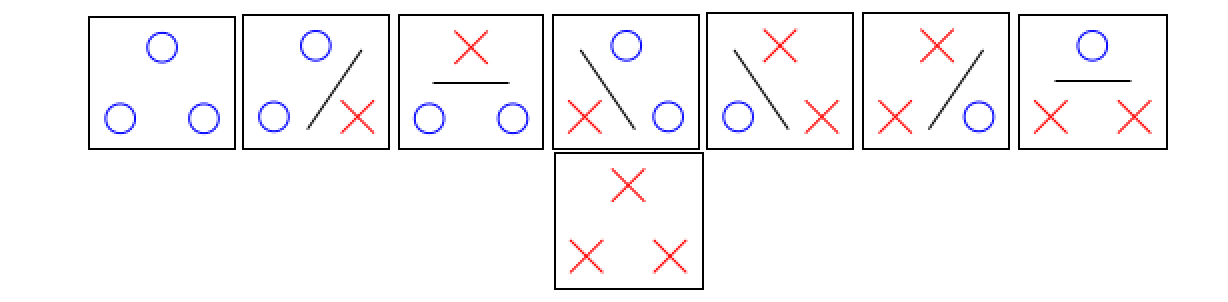
\includegraphics[width=0.9\textwidth]{images/Bias-Variance Tradeoff_05.png}           
            \end{center}
            \item $\mathbf{VC(C)< 4}$, we must show that it does not exists a set of 4 points which can be shattered by a linear classifier, consider the following cases:
            \begin{itemize}
                \item 4 aligned: alternating the instances from + to - we cannot shatter them
                \item 3 aligned: alternating the instances from + to - of the 3 aligned we cannot shatter them
                \item 4 on a convex hull: label the points on the two diagonals with opposite classes, we cannot shatter them
                \item 3 on a convex hull (triangle), 4-th inside it: the ones on the triangle same label, the inside one has the opposite label
            \end{itemize}
            \begin{center}
                
\includegraphics[width=0.9\textwidth]{images/Bias-Variance Tradeoff_06.png}           
            \end{center}
        \end{itemize}
    \end{minipage}}

    How many samples do you need to guarantee that the rectangle classifier provides you with an error larger than $\epsilon=0.1$ with probability smaller than $\delta=0.2$?

    \fbox{\begin{minipage}{\linewidth}
        Use the formula for VC:

        \vspace{1em}
        $
        N\geq\frac{1}{\epsilon}\left(
            4\log_2\left(\frac{2}{\delta}\right)+8VC(H)\log_2\left(\frac{13}{2}\right)
        \right)
        \\
        N\geq 10(4\log_2(10)+8*4\log_2(130))
        \\
        N\geq \left\lceil 10(4*4+32*7) \right\rceil
        \\
        N\geq 2400
        $

        \vspace{1em}
    \end{minipage}}

\subsubsection{PAC bound}
    Consider the hypothesis space of the decision trees with attributes with $n=4$ binary features with at most $k=10$ leaves (in this case you have less than $n^{k-1}2^{2k-1}$ different trees) and the problem of binary classification.\\
    Suppose you found a learning algorithm which is able to perfectly classify a training set of $N=1000$ samples. What is the lowest error $\epsilon$ you can guarantee to have with probability greater than $1-\delta=0.95$? How many samples do you need to halve this error?

    \fbox{\begin{minipage}{\linewidth}
        $$N\geq\frac{1}{\epsilon}\left(\ln|H|+\ln(\frac{1}{\delta})\right)$$
        We want to find $\epsilon$

        \vspace{1em}
        $
        \epsilon\geq\frac{1}{N}\left(\ln|H|+\ln(\frac{1}{\delta})\right)
        \\\cdots=\frac{1}{1000}\left(
            \ln (4^{10-1}2^{2*10-1})+\ln (\frac{1}{0.05})
        \right)
        \\\cdots=\frac{1}{1000}\left(
            \ln (4^92^{19})+\ln (\frac{1}{0.05})
        \right)
        \\\cdots=0.0286
        $

        \vspace{1em}
        To halve this error, we would need just need to double the number of samples we had originally, still requiring to have a perfect classifier on the new training set
    \end{minipage}}

    Another classifier is able only to get an error of $L_{train}(h)=0.02$ on your original training set. It is possible to use the same error bound derived in the first case? If not, derive a bound with the same probability for this case. How many samples do we need to halve the error bound?

    \fbox{\begin{minipage}{\linewidth}
        Agnostic learning since we cannot use the previous bound, the classifier is not able to perfectly classify all the points in the training set ($L_{train}\neq 0$)
        $$Pr(\exists\,\,h\,\in H|L_{true}(h)-L_{train}(h)>\epsilon)\leq|H|e^{-2N\epsilon^2}$$
        Thus the error bound is
        $$err=L_{true}=L_{train}+\epsilon\leq\underset{Bias}{\underbrace{L_{train}(h)}}+\underset{Variance}{\underbrace{\sqrt{\frac{\ln|H|+\ln\frac{1}{\delta}}{2N}}}}$$
        $
        \\\cdots=0.02+\sqrt{\frac{0.0286}{2}}
        \\\cdots=0.1397
        $

        \vspace{1em}
        To halve this error we solve for $N$
        $$L_{train}(h)+\sqrt{\frac{\ln|H|+\ln\frac{1}{\delta}}{2N}}\leq \frac{0.1397}{2}\Rightarrow N\geq 5766.34\sim 5767$$
    \end{minipage}}

\subsection{Kernel methods}
\subsubsection{SVM}
    Consider the linear two-class SVM classifier defined by the parameters $w=[2\,\,1],\,\,b=1$. Is the point $x_1=[-2\,\,4]$ a support vector?

    \fbox{\begin{minipage}{\linewidth}
        A point is a support vector if $|w^Tx+b|\leq 1$
        $$|w^Tx+b|=|-4+4+1|=1$$
        So it is a support vector
    \end{minipage}}

    Provide the analytical formula of the boundary and the margins.

    \fbox{\begin{minipage}{\linewidth}
        $$
        \begin{cases}
            2x_1+1x_2+1=0\text{\hspace{1em}(boundary)}\\
            2x_1+x_2+1=1\text{\hspace{1.5em}(positive margin)}\\
            2x_1+x_2+1=-1\text{\hspace{0.75em}(negative margin)}\\
        \end{cases}
        $$
    \end{minipage}}

    Give an example of a point which is on the boundary of the SVM

    \fbox{\begin{minipage}{\linewidth}
        A point on the boundary has to satisfy $w^Tx+b=0$, we can consider $x_{11}=0$ and solve
        $$2*0+1x_{22}+1=0\rightarrow x_{22}=-1$$
        So $x=[0\,\,-1]$ is on the boundary
    \end{minipage}}

    How the point $x_2=[3\,\,-1]$ is classified according to the trained SVM?

    \fbox{\begin{minipage}{\linewidth}
        $$w^Tx_2+b=2*3-1*1+1=6$$
        As binary classifier and positive, the point is classified in the positive class
    \end{minipage}}

    Assume to collect a new sample $x_3=[-1\,\,2]$ in the negative class, do we need to retrain the SVM?

    \fbox{\begin{minipage}{\linewidth}
        $$w^Tx_3+b=-2+2+1=1$$
        The point is missclassified, which means that $x_3$ would be a support vector thus we need to retrain the model
    \end{minipage}}

    Let us suppose we collect new data that make the classification task not linearly separable. How would you change the SVM model to deal with the task?

    \fbox{\begin{minipage}{\linewidth}
        We could either consider a soft-margin SVM or a different kernel function. In any case we should retrain the model to update the paramaters accordingly.
    \end{minipage}}

\subsection{Markov Decision Processes}
\subsubsection{Examples of MDPs}
    For each of the following dichotomies in MDP modeling provide examples of problems with the listed characteristics:
    \begin{tabularx}{\linewidth}{X|X|X|X}
        \toprule
        \endfirsthead
        \toprule
        \textbf{} & \textbf{} & \textbf{} & \textbf{}\\
        \midrule
        \endhead
        \footnotesize [Continues on next page]
        \endfoot
        \bottomrule
        \endlastfoot
        %body
        \textbf{Finite actions} & Robotic navigation (up, down, left, right) & \textbf{Infinite actions} & Pole balancing with continuous space applied force\\ \midrule
        \textbf{Deterministic transitions} & Chess (given the opponent strategy) & \textbf{Stochastic transitions} & Blackjack\\ \midrule
        \textbf{Deterministic rewards} & Robot navigation (0 everywhere, 1 in the exit point) & \textbf{Stochastic rewards} & Ad banner allocation (depending on clicks)\\ \midrule
        \textbf{Finite horizon} & Carcassone (finite number of tiles) & \textbf{Infinite horizon} & Stock exchange\\ \midrule
        \textbf{Indefinite horizon} & Chess & & \\ \midrule
        \textbf{Stationary environment} & Robotic navigation & \textbf{Non-stationary environment} & Every game with another learner playing
    \end{tabularx}

\subsubsection{Value function}
    Consider the MDP with $\alpha=0.3,\,\,\beta=0.5,\,\,\gamma=1,\,\,r_{search}=2,\,\,r_{wait}=0$ and the following policy:
    $$\pi(s|H)=1$$
    $$\pi(s|L)=0.5$$
    $$\pi(r|L)=0.5$$
    Compute the value function where the MDP stops after two steps
    \begin{center}
        \begin{tikzpicture}[shorten >=1pt,node distance=8cm,on grid,auto]
            \node[state] (q_0) {$H$};
            \node[state] (q_1) [right=of q_0] {$L$};

            \path[->] 
            (q_0) %H%
                edge[loop above] node [swap] {wait: 1,$r_{wait}$} (q_0)
                edge[loop below] node [swap] {search: $\alpha,r_{search}$} (q_0)
                edge[out=315,in=225]  node [swap] {search: $1-\alpha,r_{search}$} (q_1)
            (q_1) %L%
                edge[loop above] node[swap] {search: $\beta,r_{search}$} (q_1)
                edge[loop below] node[swap] {wait: $1,r_{wait}$} (q_1)
                edge[out=180,in=0] node[swap] {recharge: 1,0} (q_0)
                edge[out=135,in=45] node[swap] {search: $1-\beta,-3$} (q_0)
            ;
        \end{tikzpicture}                
    \end{center}
    \fbox{\begin{minipage}{\linewidth}
        Use the Bellman expectation equation and operator
        $$V^\pi=\sum_{a \in A}\pi(a|s)\left(R(s,a)+\gamma\sum_{s'\in S}P(s'|s,a)V^\pi(s')\right)$$
        We first compute the immediate rewards, so stop at step 1 (so $P(s'|s,a)=0$ immediately)
        $$
        V^\pi=\sum_{a \in A}\pi(a|s)R(s,a)\Rightarrow
        \begin{cases}
            V^\pi(H)=\pi(s|H)R(H,s)=2\\
            V^\pi(L)=\pi(s|L)R(L,s)+\pi(r|L)R(L,r)
            \\\cdots=0.5*(\beta*2+(1-\beta)*(-3))+0.5*0
            \\\cdots=0.5*(0.5*2+0.5*(-3))
            \\\cdots=-0.25
        \end{cases}
        $$
        \begin{itemize}
            \item For $H$ as the policy only considers action $s$, only one member for the outer summation\\
            $
            V^\pi(H)=\pi(s|H)\left(
                R(H,s)+1(P(H|H,s)V^\pi(H)+P(L|H,s)V^\pi(L))
            \right)
            \\\cdots= 1\left(
                2+1(\alpha V^\pi(H)+(1-\alpha)V^\pi(L))
            \right)
            \\\cdots=2+0.3V^\pi(H)+0.7V^\pi(L)
            $\\
            Since we stop at step 2, we now consider the immediate reward and also $P(s'|s,a)=0$ as we stop
            $
            \\\cdots=2+0.3*2+0.7*(-0.25)=2.425
            $
            \item For $L$ we consider two terms in the outer summation\\
            $
            V^\pi(L)=\pi(s|L)\left(
                R(L,s)+1(P(L|L,s)V^\pi(L)+P(H|L,s)V^\pi(H))
            \right)
            \\+\pi(r|L)\left(
                R(L,r)+1(P(L|L,r)V^\pi(L)+P(H|L,r)V^\pi(H))
            \right)
            \\\cdots=0.5\left(
                \beta*2+(1-\beta)*(-3)+1(\beta V^\pi(L)+(1-\beta) V^\pi(H))
            \right)+0.5\left(
                0+1(0+1V^\pi(H))
            \right)
            \\\cdots=0.5\left(
                0.5*2+0.5*(-3)+0.5V^\pi(L)+0.5V^\pi(H)
            \right)+0.5V^\pi(H)
            \\\cdots=-0.25+0.25V^\pi(L)+0.25V^\pi(H)+0.5V^\pi(H)
            $\\
            Since we stop at step 2, we now consider the immediate reward and also $P(s'|s,a)=0$ as we stop
            $
            \\\cdots=-0.25+0.25*(-0.25)+0.75*2=1.1875
            $
        \end{itemize}
    \end{minipage}}

    What happens if we consider a discount factor of $\gamma=0.5$?

    \fbox{\begin{minipage}{\linewidth}
        Use the Bellman expectation equation and operator
        $$V^\pi=\sum_{a \in A}\pi(a|s)\left(R(s,a)+\gamma\sum_{s'\in S}P(s'|s,a)V^\pi(s')\right)$$
        The immediate rewards are unchanged
        $$
        V^\pi=\sum_{a \in A}\pi(a|s)R(s,a)\Rightarrow
        \begin{cases}
            V^\pi(H)=\pi(s|H)R(H,s)=2\\
            V^\pi(L)=\pi(s|L)R(L,s)+\pi(r|L)R(L,r)=-0.25
        \end{cases}
        $$
        \begin{itemize}
            \item For $H$ as the policy only considers action $s$, only one member for the outer summation\\
            $
            V^\pi(H)=\pi(s|H)\left(
                R(H,s)+0.5(P(H|H,s)V^\pi(H)+P(L|H,s)V^\pi(L))
            \right)
            \\\cdots= 1\left(
                2+0.5(\alpha V^\pi(H)+(1-\alpha)V^\pi(L))
            \right)
            \\\cdots=2+0.5(0.3V^\pi(H)+0.7V^\pi(L))
            $\\
            Since we stop at step 2, we now consider the immediate reward and also $P(s'|s,a)=0$ as we stop
            $
            \\\cdots=2+0.5(0.3*2+0.7*(-0.25))=2.2125
            $
            \item For $L$ we consider two terms in the outer summation\\
            $
            V^\pi(L)=\pi(s|L)\left(
                R(L,s)+0.5(P(L|L,s)V^\pi(L)+P(H|L,s)V^\pi(H))
            \right)
            \\+\pi(r|L)\left(
                R(L,r)+0.5(P(L|L,r)V^\pi(L)+P(H|L,r)V^\pi(H))
            \right)
            \\\cdots=0.5\left(
                \beta*2+(1-\beta)*(-3)+0.5(\beta V^\pi(L)+(1-\beta) V^\pi(H))
            \right)+0.5\left(
                0+0.5(0+1V^\pi(H))
            \right)
            \\\cdots=0.5\left(
                0.5*2+0.5*(-3)+0.5(0.5V^\pi(L)+0.5V^\pi(H))
            \right)+0.25V^\pi(H)
            \\\cdots=-0.25+0.125V^\pi(L)+0.125V^\pi(H)+0.25V^\pi(H)
            $\\
            Since we stop at step 2, we now consider the immediate reward and also $P(s'|s,a)=0$ as we stop
            $
            \\\cdots=-0.25+0.125*(-0.25)+0.375*2=0.46875
            $
        \end{itemize}
        Clearly the discounted value for the states is lower than the not discounted one, in the case we consider an MDP with finite time horizon.
    \end{minipage}}

    Compute the action-value function for each action value pair in the case the MDP stops after a single step

    \fbox{\begin{minipage}{\linewidth}
        Use the Bellman expectation equation and operator
        $$Q^\pi(s,a)=R(s,a)+\gamma\sum_{s' \in S}P(s'|s,a)\sum_{a' \in A}\pi(a'|s')Q^\pi(s',a')$$
        If it stops at the first step, we are computing the instantaneous reward
        $$
        Q^\pi(s,a)=R(s,a)\Rightarrow
        \begin{cases}
            Q(L,w)=1*0=0\\
            Q(L,s)=\beta*2+(1-\beta)*(-3)=-0.5\\
            Q(L,r)=1*0=0\\
            Q(H,w)=1*0=0\\
            Q(H,s)=\alpha*2+(1-\alpha)*2=2
        \end{cases}
        $$
    \end{minipage}}

\subsubsection{Bellman expectation equation for $V$}
    Provide the formulation of the Bellman expectation equation for $V$ equations for the MDP
    \begin{center}
        \begin{tikzpicture}[shorten >=1pt,node distance=8cm,on grid,auto]
            \node[state] (q_0) {$H$};
            \node[state] (q_1) [right=of q_0] {$L$};
    
            \path[->] 
            (q_0) %H%
                edge[loop above] node [swap] {wait: 1,$r_{wait}$} (q_0)
                edge[loop below] node [swap] {search: $\alpha,r_{search}$} (q_0)
                edge[out=315,in=225]  node [swap] {search: $1-\alpha,r_{search}$} (q_1)
            (q_1) %L%
                edge[loop above] node[swap] {search: $\beta,r_{search}$} (q_1)
                edge[loop below] node[swap] {wait: $1,r_{wait}$} (q_1)
                edge[out=180,in=0] node[swap] {recharge: 1,0} (q_0)
                edge[out=135,in=45] node[swap] {search: $1-\beta,-3$} (q_0)
            ;
        \end{tikzpicture}                
    \end{center}
    With $\alpha=0.2,\,\,\beta=0.1,\,\,r_{search}=2,\,\,r_{wait}=0,\,\,\gamma=0.9$ and in the case we consider the policy:
    $$\pi(H|s)=1$$
    $$\pi(L|r)=1$$
    \fbox{\begin{minipage}{\linewidth}
        Use the Bellman expectation equation and operator
        $$V^\pi=\sum_{a \in A}\pi(a|s)\left(R(s,a)+\gamma\sum_{s'\in S}P(s'|s,a)V^\pi(s')\right)$$
        $$V^\pi=R^\pi+\gamma P^\pi V^\pi$$
        We obtain

        $
        V^\pi(H)=\pi(H|s)\left(
            R(H,s)+0.9(P(H|H,s)V^\pi(H)+P(L|H,s)V^\pi(L))
        \right)
        \\\cdots=2+0.9(\alpha V^\pi(H)+(1-\alpha)V^\pi(L))
        \\\cdots=2+0.9(0.2V^\pi(H)+0.8V^\pi(L))\\
        V^\pi(L)=\pi(L|r)\left(
            R(L,r)+0.9(P(L|L,r)V^\pi(L)+P(H|L,r)V^\pi(H))
        \right)
        \\\cdots=0+0.9(0+1V^\pi(H))
        \\\cdots=0+0.9V^\pi(H)
        $

        Which in matrix form:
        $$
        V^\pi=
        \begin{bmatrix}
            2\\
            0
        \end{bmatrix}
        +0.9
        \begin{bmatrix}
            0.2 & 0.8\\
            1 & 0
        \end{bmatrix}
        V^\pi
        $$
    \end{minipage}}
    
\subsubsection{Transition matrix, value and action-value functions}
    \begin{center}
        \begin{tikzpicture}[shorten >=1pt,node distance=6cm,on grid,auto]
            \node[state] (q_0) {$s_1$ Good shape};
            \node[state] (q_2) [below right=of q_0] {$s_3$ Broken};
            \node[state] (q_1) [above right=of q_2] {$s_2$ Deteriorating};

            \path[->] 
            (q_0) %s_1%
                edge[loop above] node[swap] {Maintain: $1,0$} (q_0)
                edge[loop right] node[swap] {Ignore: $0.5,1$} (q_0)
                edge[out=20,in=160] node[swap] {Ignore: $0.5,0.5$} (q_1)
            (q_1) %s_2%
                edge[loop above] node[swap] {Maintain: $0.1,-1$} (q_1)
                edge[out=135,in=45] node[swap] {Maintain: $0.9,0$} (q_0)
                edge[loop below] node[swap] {Ignore: $0.5,0.5$} (q_1)
                edge[out=225,in=45] node[swap] {Ignore: $0.5,0$} (q_2)
            (q_2) %s_3%
                edge[loop below] node[swap] {Ignore: $1,0$} (q_2)
                edge[loop left] node[swap] {Maintain: $0.8,0$} (q_2)
                edge[out=135,in=315] node[below left] {Maintain: $0.2,0$} (q_0)
            ;
        \end{tikzpicture}                
    \end{center}
    Provide the transition matrix for the policy $\pi(I|s_1)=1,\,\,\pi(M|s_2)=1,\,\,\pi(M|s_3)=1$

    \fbox{\begin{minipage}{\linewidth}
        We model a row as $[(S_i,a_1,S_0) (S_i,a_1,S_1) \cdots]$ and a column as $[(S_i,a_0,S_j) (S_i,a_1,S_j) \cdots]^T$.\\
        We follow this order for the actions: Ignore, Maintain
        $$
        P=
        \begin{bmatrix}
            0.5 & 0.5 & 0\\
            1 & 0 & 0\\
            0 & 0.5 & 0.5\\
            0.9 & 0.1 & 0\\
            0 & 0 & 1\\
            0.2 & 0 & 0.8
        \end{bmatrix}
        $$
        The policy tells us to keep the rows 1, 4 and 6:
        $$
        P=
        \begin{bmatrix}
            0.5 & 0.5 & 0\\
            0.9 & 0.1 & 0\\
            0.2 & 0 & 0.8
        \end{bmatrix}
        $$
    \end{minipage}}

    Provide the expected instantaneous reward for the previous policy

    \fbox{\begin{minipage}{\linewidth}
        We consider only those three transictions, the instantaneous rewards are
        $$
        R=
        \begin{bmatrix}
            0.5*1+0.5*0.5\\
            0.1*-1+0.9*0\\
            0.8*0+0.2*0
        \end{bmatrix}
        =
        \begin{bmatrix}
            0.75\\
            -0.1\\
            0
        \end{bmatrix}
        $$
    \end{minipage}}

    Compute the value function for the previous policy in the case the MDP stops after two steps with $\gamma=1$

    \fbox{\begin{minipage}{\linewidth}
        Use the Bellman expectation equation and operator
        $$V^\pi=\sum_{a \in A}\pi(a|s)\left(R(s,a)+\gamma\sum_{s'\in S}P(s'|s,a)V^\pi(s')\right)$$
        \begin{itemize}
            \item $
            V^\pi(s_1)=R(s_1,I)+0.5V^\pi(s_1)+0.5V^\pi(s_2)
            \\\cdots=0.75+0.5V^\pi(s_1)+0.5V^\pi(s_2)
            \\\cdots=0.75+0.5*0.75+0.5*(-0.1)=1.075
            $
            \item $
            V^\pi(s_2)=R(s_2|M)+0.1V^\pi(s_1)+0.9V^\pi(s_2)
            \\\cdots=-0.1+0.9*0.75+0.1*(-0.1)=0.565
            $
            \item $
            V^\pi(s_3)=R(s_3|M)+0.2V^\pi(s_1)+0.8V^\pi(s_2)
            \\\cdots=0+0.2*0.75+0=0.15
            $
        \end{itemize}
    \end{minipage}}

    Compute the action-value function for each state-action pair in the case the MDP stops after a single step

    \fbox{\begin{minipage}{\linewidth}
        Use the Bellman expectation equation and operator
        $$Q^\pi(s,a)=R(s,a)+\gamma\sum_{s' \in S}P(s'|s,a)\sum_{a' \in A}\pi(a'|s')Q^\pi(s',a')$$
        If it stops at the first step, we are computing the instantaneous reward
        $$
        Q^\pi(s,a)=R(s,a)\Rightarrow
        \begin{cases}
            Q(s_1,I)=0.5*1+0.5*0.5=0.75\\
            Q(s_1,M)=1*0=0\\
            Q(s_2,I)=0.5*0.5+0.5*0=0.25\\
            Q(s_2,M)=0.1*(-1)+0.9*0=-0.1\\
            Q(s_3,I)=1*0=0\\
            Q(s_3,M)=0.8*0+0.2*0=0
        \end{cases}
        $$
    \end{minipage}}

\subsubsection{MDP $\gamma$}
    Consider an MDP with 3 states and 3 actions. Applying the policy $\pi$ we have the following action-value function $Q(s,a)$ when we consider discount factors $\gamma$:
    \begin{tabularx}{\linewidth}{X|c c c|c c c|c c c}
        \toprule
        \endfirsthead
        \toprule
        \midrule
        \endhead
        \midrule
        \footnotesize [Continues on next page]
        \endfoot
        \bottomrule
        \endlastfoot
        & & $\gamma=0.9$ & & & $\gamma=0.95$ & & & $\gamma=0.99$ &\\ \midrule
        & d & so & cm & d & so & cm & d & so & cm\\ \midrule
        s1 & 35 & 25 & 0 & 95 & 90 & 0 & 780 & 785 & 0\\ \midrule
        s2 & 55 & 0 & 45 & 120 & 0 & 125 & 810 & 0 & 825\\ \midrule
        s3 & 165 & 0 & 0 & 240 & 0 & 0 & 940 & 0 & 0
    \end{tabularx}
    Provide the optimal policy $\pi^*$ for each discount factor $\gamma$.

    \fbox{\begin{minipage}{\linewidth}
        Assuming that the policy $\pi$ is explorative enough (visits all states and tries all available actions) the optimal policy is the one which maximize the value function in each state:
        $$\pi^*(0.9)=(d,d,d)$$
        $$\pi^*(0.95)=(d,cm,d)$$
        $$\pi^*(0.99)=(so,cm,d)$$
    \end{minipage}}

    What is the expected reward for $\pi^*$ if the initial state distribution is (0.4, 0.4, 0.2)?

    \fbox{\begin{minipage}{\linewidth}
        The expected reward $R(\gamma)$ is given by $p^TV^*(\gamma)$
        $$R(0.9)=(0.4,0.4,0.2)^T(35,55,165)=14+22+33=69$$
        $$R(0.95)=(0.4,0.4,0.2)^T(95,125,240)=136$$
        $$R(0.99)=(0.4,0.4,0.2)^T(785,825,940)=832$$
    \end{minipage}}

    Which $\gamma$ would you choose for this specific problem?

    \fbox{\begin{minipage}{\linewidth}
        This question does not make sense, the discount factor is not a parameter that should be chosen by the learner, but a characteristic of the MDP. The use of different values of $\gamma$ depends on the fact that the problem requires to be more far-sighted or myopic.
    \end{minipage}}

\subsection{Reinforcement Learning}
\subsubsection{MC and TD for state-value}
    Evaluate the value for the MDP with states $S=\{A,B,C\}$, $C$ is terminal with reward zero then, actions $A=\{h,r\}$ given the policy $\pi$ and the following trajectories:

    \vspace{1em}
    $(A,h,3)\rightarrow(B,r,2)\rightarrow(B,h,1)\rightarrow(C)$\\
    $(A,h,2)\rightarrow(A,h,1)\rightarrow(C)$\\
    $(B,r,1)\rightarrow(A,h,1)\rightarrow(C)$
    
    \vspace{1em}
    Can you tell without computing anything if by resorting to MC every-visit and first-visit approach you will have different results?

    \fbox{\begin{minipage}{\linewidth}
        Yes, in the first episode $B$ repeated twice, and in the third $A$ repeated twice, so different estimate
    \end{minipage}}

    Compute the values with the two aforementioned methods

    \fbox{\begin{minipage}{\linewidth}
        For MC:
        $$V(s_t)\leftarrow V(s_t)+\alpha (v_t-V(s_t))$$
        \begin{itemize}
            \item \textbf{First visit}
            $$
            V(A)=
            \begin{cases}
                \mathbf{(A,h,3)\rightarrow(B,r,2)\rightarrow(B,h,1)\rightarrow(C)\Rightarrow 6}\\
                \mathbf{(A,h,2)\rightarrow(A,h,1)\rightarrow(C)\Rightarrow 3}\\
                (B,r,1)\rightarrow\mathbf{(A,h,1)\rightarrow(C)\Rightarrow 1}\\
            \end{cases}
            = 10/3
            $$
            $$
            V(B)=
            \begin{cases}
                (A,h,3)\rightarrow\mathbf{(B,r,2)\rightarrow(B,h,1)\rightarrow(C)\Rightarrow 3}\\
                (A,h,2)\rightarrow(A,h,1)\rightarrow(C)\mathbf{\Rightarrow 0,\,\,not\,\,considered}\\
                \mathbf{(B,r,1)\rightarrow(A,h,1)\rightarrow(C)\Rightarrow 2}\\
            \end{cases}
            = 5/2
            $$
            \item \textbf{Every visit}
            $$
            V(A)=
            \begin{cases}
                \mathbf{(A,h,3)\rightarrow(B,r,2)\rightarrow(B,h,1)\rightarrow(C)\Rightarrow 6}\\
                \begin{cases}
                    \mathbf{(A,h,2)\rightarrow(A,h,1)\rightarrow(C)\Rightarrow 3}\\
                    (A,h,2)\rightarrow\mathbf{(A,h,1)\rightarrow(C)\Rightarrow 1}
                \end{cases}\\
                (B,r,1)\rightarrow\mathbf{(A,h,1)\rightarrow(C)\Rightarrow 1}
            \end{cases}
            = 11/4
            $$
            $$
            V(B)=
            \begin{cases}
                \begin{cases}
                    (A,h,3)\rightarrow\mathbf{(B,r,2)\rightarrow(B,h,1)\rightarrow(C)\Rightarrow 3}\\
                    (A,h,3)\rightarrow(B,r,2)\rightarrow\mathbf{(B,h,1)\rightarrow(C)\Rightarrow 1}
                \end{cases}\\
                (A,h,2)\rightarrow(A,h,1)\rightarrow(C)\mathbf{\Rightarrow 0,\,\,not\,\,considered}\\
                \mathbf{(B,r,1)\rightarrow(A,h,1)\rightarrow(C)\Rightarrow 2}
            \end{cases}
            = 6/3 = 2
            $$
        \end{itemize}
    \end{minipage}}

    Assume to consider a discount factor $\gamma=1$ and compute the values resorting to TD. Assume to start from zero values for each state and $\alpha=0.1$

    \fbox{\begin{minipage}{\linewidth}
        For TD:
        $$V(s_t)\leftarrow V(s_t)+\alpha (r_{t+1}+\gamma V(s_{t+1})-V(s_t))$$
        As we start from zero values, consider transition of episode 1
        $$(A,h,3)\rightarrow(B,r,2)\rightarrow(B,h,1)\rightarrow(C)$$
        
        $(A,h,3)\rightarrow(B,h,1)$
        $$V(A)=\underset{Initially\,\,all\,\,zero\,\,for\,\,A}{\underbrace{0}}+0.1(3+1*\underset{State\,B\,\,initially\,\,zero}{\underbrace{0}}-0)=0.3$$

        $(B,r,2)\rightarrow(B,h,1)$
        $$V(B)=0+0.1(2+1*0-0)=0.2$$

        $(B,h,1)\rightarrow(C)$
        $$V(B)=\underset{V(B)\,\,from\,\,step\,\,before}{\underbrace{0.2}}+0.1*(1+1*0-0.2)$$
        And so on...
    \end{minipage}}

\subsubsection{MC policy evaluation, improvement with $\epsilon$-greedy}
    Consider the set of trajectories below with discount factor $\gamma=1$

    \vspace{1em}
    $(A,u,2)\rightarrow(B,d,-2)\rightarrow(A,d,-2)\rightarrow(A,u,4)\rightarrow(C)$\\
    $(A,d,1)\rightarrow(B,u,-3)\rightarrow(C)$\\
    $(A,d,7)\rightarrow(B,d,0)\rightarrow(C)$

    \vspace{1em}
    Provide the policy evaluation step according to MC first-visit.

    \fbox{\begin{minipage}{\linewidth}
        $$
        Q(A,u)=
        \begin{cases}
            \mathbf{(A,u,2)\rightarrow(B,d,-2)\rightarrow(A,d,-2)\rightarrow(A,u,4)\rightarrow(C)\Rightarrow 2}\\
            (A,d,1)\rightarrow(B,u,-3)\rightarrow(C)\mathbf{\Rightarrow not\,\,considered}\\
            (A,d,7)\rightarrow(B,d,0)\rightarrow(C)\mathbf{\Rightarrow not\,\,considered}
        \end{cases}
        = 2
        $$
        And so on...
        $$
        \begin{cases}
            Q(A,u)=-2\\
            Q(B,u)=-3\\
            Q(A,d)=\frac{2-2+7}{3}=\frac{7}{3}\\
            Q(B,d)=\frac{0+0}{2}=0
        \end{cases}
        $$
    \end{minipage}}

    Provide the policy improvement step, i.e., the policy that the algorithm will deploy at the next iteration.

    \fbox{\begin{minipage}{\linewidth}
        In MC policy iteration we have to ensure sufficient exploration by deploying $\epsilon$-greedy policy, i.e.:
        $$
        \begin{cases}
            \pi(u|A)=\epsilon\\
            \pi(d|A)=1-\epsilon\\
            \pi(u|B)=\epsilon\\
            \pi(d|B)=1-\epsilon
        \end{cases}
        $$
    \end{minipage}}

    Do you think the results would have changed with MC every-visit evaluation?

    \fbox{\begin{minipage}{\linewidth}
        The only state-action pair that occurs more than once in single trajectory is $(A,u)$, so:
        $$
        Q(A,u)=\frac{2+4}{2}=3
        $$
        And since $Q(A,u)>Q(A,d)$ the $\epsilon$-greedy policy will change with $\pi(u|A)=1-\epsilon$ and $\pi(d|A)=\epsilon$
    \end{minipage}}

\subsubsection{SARSA}
    Conside the trajectory below, which is obtained while running the SARSA algorithm in an MDP with three states $S=\{A,B,C\}$, two actions $A=\{u,d\}$ and discount factor $\gamma=1$.
    $$(A,u,2)\rightarrow(B,d,-2)\rightarrow(A,d,-2)\rightarrow(A,u,-1)\rightarrow(B,u,-3)\rightarrow(C,d,4)\rightarrow(B)$$
    Provide a consistent guess over the policy $\pi$ that has been used to draw the latter trajectory. Do you think it is a reasonable policy?

    \fbox{\begin{minipage}{\linewidth}
        A guess:

        \vspace{1em}
        $
        \pi(u|A)=2/3\hspace{2em}\pi(d|A)=1/3\\
        \pi(u|B)=1/2\hspace{2em}\pi(d|B)=1/2\\
        \pi(u|C)=0\hspace{3em}\pi(d|C)=1
        $

        \vspace{1em}
        We do not have enough data to reliably estimate the policy $\pi$. On the one hand, it is unreasonable to have a deterministic policy in the state C, as we should guarantee sufficient exploration for the SARSA algorithm to converge to the optimal policy. On the other hand, the policy in the states A, B seems to be overly randomized to be an $\epsilon$-greedy policy.
    \end{minipage}}

    Provide the policy evaluation step according to SARSA by considering zero initial value $Q(s,a)=0$ for every state-action pair, and learning rate $\alpha=0.5$

    \fbox{\begin{minipage}{\linewidth}
        SARSA uses TD:
        $$Q(s,a)\leftarrow Q(s,a)+\alpha(r+\gamma Q(s',a')-Q(s,a))$$
        Starting from null values, follow the order of the episodes, we have:

        \vspace{1em}
        $
        Q^\pi(A,u)=0+0.5(2+1Q^\pi(B,d)-0)=0.5*2=1\\
        Q^\pi(B,d)=0+0.5(-2+Q^\pi(A,d)-0)=-1\\
        Q^\pi(A,d)=0+0.5(-2+Q^\pi(A,u)-0)=0.5(-2+1)=-0.5\\
        Q^\pi(A,u)=1+0.5(-1+Q^\pi(B,u)-1)=0\\
        Q^\pi(B,u)=0+0.5(-3+Q^\pi(C,d)-0)=-1.5\\
        Q^\pi(C,d)=0+0.5(4+0-0)=2
        $
    \end{minipage}}

    Provide the policy improvement step, i.e., the policy $\pi'$ that the algorithm will deploy at the next iteration.

    \fbox{\begin{minipage}{\linewidth}
        With the SARSA algorithm we have to ensure sufficient exploration, e.g. by deploying $\epsilon$-greedy policy ($1-\epsilon$ probability to choose greedy action), thus we have:

        \vspace{1em}
        $
        \pi(u|A)=1-\epsilon\hspace{2em}\pi(d|A)=\epsilon\\
        \pi(u|B)=\epsilon\hspace{3.5em}\pi(d|B)=1-\epsilon\\
        \pi(u|C)=\epsilon\hspace{3.5em}\pi(d|C)=1-\epsilon
        $
    \end{minipage}}

\subsubsection{Q-learning}
    Consider the following episode obtained by an agent interacting with an MDP having two states $S=\{A,B\}$ and two actions $A=\{l,r\}$
    $$(A,l,1)\rightarrow(A,l,1)\rightarrow(A,r,0)\rightarrow(B,r,10)\rightarrow(B,l,0)\rightarrow(A,r,0)\rightarrow(B,l,0)\rightarrow(A)$$
    Execute the Q-learning algorithm on the given episode considering initial state-action values $Q(S,a)=0$ for every stat-action pair, learning rate $\alpha=0.5$ and discount factor $\gamma=1$

    \fbox{\begin{minipage}{\linewidth}
        Q-learning:
        $$Q(s,a)\leftarrow Q(s,a)+\alpha(r+\gamma \max_{a'\in A}Q(s',a')-Q(s,a))$$
        
        a)\hspace{1em}$(A,l,1)\rightarrow(A,l,1)$
        $$Q(A,l)=0+0.5(1+1*0-0)=0.5$$

        b)\hspace{1em}$(A,l,1)\rightarrow(A,r,0)$
        $$Q(A,l)=0.5+0.5(1+1*0.5-0.5)=1$$

        c)\hspace{1em}$(A,r,0)\rightarrow(B,r,10)$
        $$Q(A,r)=0+0.5(0+1*\underset{Max\,\,value\,\,from\,\,state\,\,B\,\,is\,\,0}{\underbrace{0}}-0)=0$$

        d)\hspace{1em}$(B,r,10)\rightarrow(B,l,0)$
        $$Q(B,r)=0+0.5(10+1*0-0)=5$$

        e)\hspace{1em}$(B,l,0)\rightarrow(A,r,0)$
        $$Q(B,l)=\underset{Q(B,l)\,\,0\,\,still}{\underbrace{0}}+0.5(0+1*\underset{Max\,\,from\,\,A\,\,is\,\,Q(A,l)}{\underbrace{1}}-0)=0.5$$

        f)\hspace{1em}$(A,r,0)\rightarrow(B,l,0)$
        $$Q(A,r)=0+0.5(0+1*\underset{Q(B,r)}{\underbrace{5}}-0)=2.5$$

        g)\hspace{1em}$(B,l,0)\rightarrow(A)$
        $$Q(B,l)=0.5+0.5(0+1*2.5-0.5)=1.5$$
        Result:
        $$
        \begin{cases}
            Q(A,l)=1\\
            Q(A,r)=2.5\\
            Q(B,l)=1.5\\
            Q(B,r)=5
        \end{cases}
        $$
    \end{minipage}}

    Provide the best policy according to the output of Q-learning

    \fbox{\begin{minipage}{\linewidth}
        We select greedy policy $\pi(S)\in\arg\max_{a\in\{l,r\}}Q(S,a)$ w.r.t. the state-action values obtained with Q-learning, which gives $\pi(A)=r,\,\,\pi(B)=r$
    \end{minipage}}

    Do you think the agent fully exploited the policy learned in the episode above? Make a consistent guess with the available information

    \fbox{\begin{minipage}{\linewidth}
        Since at the steps a), b), \textbf{(the action chosen for A is not r)} and e) g) \textbf{(the action chosen for B is not r)} the agent is not choosing the action that is maximizing the current estimate of the Q values, we can infer that the episode does involve some exploration
    \end{minipage}}

\subsubsection{Model MDP}
    We are given an Heating, Ventilation, and Air Conditioning (HVAC) in which the states are cold (c), medium (m), warm (w) temperature. We can perform three actions: heat(h), refrigerate (r) and do nothing (d). Assume to have the following partial episodes for the HVAC functioning
    $$(c,d,0)\rightarrow(c,h,1)\rightarrow(m,h,1)\rightarrow(m,h,-1)\rightarrow(w,r,1)\rightarrow(m,.,.)\rightarrow\cdots$$
    $$(m,r,-2)\rightarrow(c,h,-2)\rightarrow(c,h,1)\rightarrow(m,h,1)\rightarrow(m,h,1)\rightarrow(w,.,.)\cdots$$
    where a tuple $(S,A,R)$ corresponds to state, action and reward.\\
    Model it as an MDP.

    \fbox{\begin{minipage}{\linewidth}
        \begin{center}
            \begin{tikzpicture}[shorten >=1pt,node distance=5cm,on grid,auto]
                \node[state] (q_0) {$C$};
                \node[state] (q_1) [right=of q_0] {$M$};
                \node[state] (q_2) [right=of q_1]{$W$};
    
                \path[->] 
                (q_0) %C%
                    edge[loop left] node [swap] {d: 1,0} (q_0)
                    edge[out=45,in=135]  node [swap] {h: 2/3,1} (q_1)
                    edge[loop above] node[swap] {h: 1/3,-2} (q_0)
                (q_1) %M%
                    edge[loop above] node[swap] {h: 2/4,1} (q_1)
                    edge[out=45,in=135] node[swap] {h: 1/4,-1} (q_2)
                    edge[out=25,in=155] node[swap] {h: 1/4,1} (q_2)
                    edge[out=225,in=315] node[swap] {r: 1,-1} (q_0)
                (q_2) %W%
                    edge[out=225,in=315] node[swap] {r: 1,1} (q_1)
                ;
            \end{tikzpicture}                
        \end{center}
        Since two edges $M\rightarrow W$ through h, we merge the edges
        \begin{center}
            \begin{tikzpicture}[shorten >=1pt,node distance=5cm,on grid,auto]
                \node[state] (q_0) {$C$};
                \node[state] (q_1) [right=of q_0] {$M$};
                \node[state] (q_2) [right=of q_1]{$W$};
    
                \path[->] 
                (q_0) %C%
                    edge[loop left] node [swap] {d: 1,0} (q_0)
                    edge[out=45,in=135]  node [swap] {h: 2/3,1} (q_1)
                    edge[loop above] node[swap] {h: 1/3,-2} (q_0)
                (q_1) %M%
                    edge[loop above] node[swap] {h: 1/2,1} (q_1)
                    edge[out=45,in=135] node[swap] {h: 1/2,0} (q_2)
                    edge[out=225,in=315] node[swap] {r: 1,-1} (q_0)
                (q_2) %W%
                    edge[out=225,in=315] node[swap] {r: 1,1} (q_1)
                ;
            \end{tikzpicture}                
        \end{center}
    \end{minipage}}

    Can you tell if the reward of this process is stochastic or deterministic? And what about the transitions?

    \fbox{\begin{minipage}{\linewidth}
        The transitions are stochastic since some of the actions are leading to two different new states (e.g. action h in the state C). The reward is stochastic as well since heating in the M state provided once the reward 1 and once -1
    \end{minipage}}

    Assuming we want to evaluate the performance of the HVAC, tell which kind of problem we are in and suggest a technique to solve it

    \fbox{\begin{minipage}{\linewidth}
        This setting suggests it is an MDP prediction problem, either using directly the original episodes (sing MC or TD) or one might use the estimated model and use DP techniques to solve it in an exact way, due to the limited dimension of the problem
    \end{minipage}}

\subsection{ Multi-Armed Bandit}
\subsubsection{Minimum regret}
    Write the formula for the minimum regret we might have on average over $T=[e^{10}]$ time steps in the case we have a stochastic MAB with 3 arms and expected rewards:

    $R(a_1)=0.2$\\
    $R(a_2)=0.4$\\
    $R(a_3)=0.7$

    and each distribution $R(a_i)$ is a Bernoulli\\
    Not that the KL divergence for Bernoulli variables with means $p$ and $q$ is:
    $$KL(p,q)=p\log(\frac{p}{q})+(1-p)\log(\frac{(1-p)}{(1-q)})$$
    Is it possible that your algorithm achieves lower regret? If so, provide an example

    \fbox{\begin{minipage}{\linewidth}
        As we consider rewards, the optimal arm is $a_3$ with 0.7.\\
        Use the formula, if we assume that T is sufficiently large, we have:
        $$\lim_{T\rightarrow \infty}L_T=R_T\geq \log T\sum_{a_i\in A:\Delta_i>0}\frac{\Delta_i}{KL(R(a_i),R(a^*))}$$
        So:
        $$R_T\geq \log e^{10}\left(
            \frac{0.7-0.2}{KL(0.2,0.7)}
            +\frac{0.7-0.4}{KL(0.7-0.4)}
        \right)=\cdots=25.1528$$
        We might violate our lower bounds in some cases:
        \begin{itemize}
            \item If we consider a subset of MAB settings
            \item If we consider a single realization of rewards
        \end{itemize}
    \end{minipage}}

\subsubsection{Regret, pseudo-regret and UCB1}
    Consider a MAB algorithm choosing the arm $a_t$ and providing the following rewards $R_t$ over a time horizon $T=10$ rounds
    \begin{tabularx}{\linewidth}{c|X X X X X X X X X X}
        \toprule
        \endfirsthead
        \toprule
        \midrule
        \endhead
        \footnotesize [Continues on next page]
        \endfoot
        \bottomrule
        \endlastfoot
        %body
        $R_{1,t}$ & \textbf{0} & 1 & 1 & 0 & \textbf{0} & 1 & 0 & 1 & \textbf{0} & 0\\
        $R_{2,t}$ & 1 & \textbf{0} & 1 & 1 & 1 & 1 & \textbf{1} & 1 & 1 & \textbf{1}\\
        $R_{3,t}$ & 0 & 1 & \textbf{0} & \textbf{0} & 0 & \textbf{0} & 1 & \textbf{0} & 1 & 1\\ \midrule
        $a_t$ & 1 & 2 & 3 & 3 & 1 & 3 & 2 & 3 & 1 & 2
    \end{tabularx}
    (only the reward for the chosen arm is revealed to the algorithm). Moreover, assume that the expected value for the three arms' reward are $\mu_1=0.3,\,\,\mu_2=0.8,\,\,\mu_3=0.6$\\
    Compute the cumulated reward, the regret and the pseudo-regret for the algorithm over the time horizon $T$. (Recall that the regret is computed over realizations, while the pseudo-regret is computed over expected values)
    
    \fbox{\begin{minipage}{\linewidth}
        \begin{itemize}
            \item Look at the table, the highlighted numbers are the rewards that we got, so cumulated rewards is just sum of those values:
            $$0+0+0+0+0+0+1+0+0+1=2$$
            \item The regret is given by the optimal reward minus the one we got:
            $$10-2=8$$
            \item We use:
            $$L_T=\sum_{a_i\in A:\Delta_i>0}\mathbb{E}[N_T(a_i)]\Delta_i$$
            At each timestamp, the $\Delta$ are the same since we consider the expected values and not the realizations. As $\mu_2$ is the maximum among the three:
            $$
            \begin{cases}
                \Delta_1=\mu_2-\mu_1=0.8-0.3=0.5\\
                \Delta_1=\mu_2-\mu_1=0.8-0.3=0\\
                \Delta_3=\mu_2-\mu_3=0.8-0.6=0.2
            \end{cases}
            $$
            So the pseudo-regret is:
            $$0.5+0+0.2+0.2+0.5+0.2+0+0.2+0.5+0=2.3$$
        \end{itemize}
    \end{minipage}}

    Compute the values for the UCB1 bounds at time 5 for the three arms. Do you think that the algorithm used in this setting can be the UCB1?

    \fbox{\begin{minipage}{\linewidth}
        $$U(a_i):=\hat{R_t}(a_i)+B_t(a_i)\geq R(a_i)$$
        For UCB1:
        $$\hat{R}_t(al)=\frac{1}{N_t(a_l)}\sum_{j=1}^{t-1}r_{a_{i_j},j}1\{a_l=a_{i_j}\},\,\forall a_i\in A$$
        $$B_t(a_l)=\sqrt{\frac{2\log t}{N_t(a_l)}},\,\forall a_l\in A$$
        So:
        $$
        \begin{cases}
            U_{1,5}=\frac{0+0}{2}+\sqrt{\frac{2\log5}{2}}\\
            U_{2,5}=\frac{0}{1}+\sqrt{\frac{2\log5}{1}}\\
            U_{3,5}=\frac{0+0}{2}+\sqrt{\frac{2\log5}{2}}
        \end{cases}
        $$
        UCB1 tries to pull the arms the same number of times (plays the one that has maximum $U$ so usually lowest $N$), therefore the arm chosen for the next round would be 2. As in timestamp 6 the arm chosen is 3, the algorithm cannot be UCB1
    \end{minipage}}

    Do you think that the algorithm used in this setting might be Thompson sampling?

    \fbox{\begin{minipage}{\linewidth}
        Since the TS has a stochastic nature, there is the chance that any possible sequence of the arms is chosen, even if with a small probability. Therefore, the algorithm run above might be TS
    \end{minipage}}

\subsubsection{Thompson sampling and UCB1}
    Consider the Thompson Sampling algorithm. Assume to have the following posterior distributions $Beta(\alpha_t,\beta_t)$ for arms $A=\{a_1,\cdots,a_5\}$ rewards, which are distributed as Bernoulli:
    \begin{enumerate}[start=1,label={- $a$\arabic{*}:}]
        \item $\alpha_t=1\hspace{1em}\beta_t=5\hspace{1em}\hat{r}(a_1)=0.63$
        \item $\alpha_t=6\hspace{1em}\beta_t=4\hspace{1em}\hat{r}(a_2)=0.35$
        \item $\alpha_t=11\hspace{1em}\beta_t=23\hspace{1em}\hat{r}(a_3)=0.16$
        \item $\alpha_t=12\hspace{1em}\beta_t=33\hspace{1em}\hat{r}(a_4)=0.22$
        \item $\alpha_t=28\hspace{1em}\beta_t=21\hspace{1em}\hat{r}(a_5)=0.7$
    \end{enumerate}

    Which arm would the TS algorithm play for the next round?

    \fbox{\begin{minipage}{\linewidth}
        $a_5$ as it has the highest sampled value ($\hat{r}$)
    \end{minipage}}

    Do you think that there is an arm that is more promising to be the best one?

    \fbox{\begin{minipage}{\linewidth}
        In TS in case of success the $\alpha_t$ is increased, so we look at arms that have $\alpha_t>\beta_t$: either $a2$ or $a5$, probably $a5$ most promising as $\alpha_t-\beta_t=7$. If there was an arm with $\beta_t=1$ it meant that it never failed: it only provided positive samples, so best one
    \end{minipage}}

    Assume we started the TS algorithm with uniform $Beta(1,1)$ priors, what would UCB1 have chosen in the case of Bernoulli rewards for the next round?
    
    \fbox{\begin{minipage}{\linewidth}
        $$U(a_i):=\hat{R_t}(a_i)+B_t(a_i)\geq R(a_i)$$
        For UCB1:
        $$\hat{R}_t(al)=\frac{1}{N_t(a_l)}\sum_{j=1}^{t-1}r_{a_{i_j},j}1\{a_l=a_{i_j}\},\,\forall a_i\in A$$
        $$B_t(a_l)=\sqrt{\frac{2\log t}{N_t(a_l)}},\,\forall a_l\in A$$
        Since we started with uniform prior and at each round we collected a success or a failure we are currently at round:
        $$t=4+8+32+43+47=134$$
        while the UCB1 upper bound $U_t(a_i)$ is of the form:
        $$U_t(a_i)=\frac{\alpha_t-1}{\alpha_t+\beta_t-2}+\sqrt{\frac{2\log t}{\alpha_t+\beta_t-2}}$$
        $$U(a_1)=\frac{0}{4}+\sqrt{
            \frac{
                2\log 134
            }{
                4
            }
        }$$
        $$\vdots$$
        \vspace{0.5em}
    \end{minipage}}

\subsubsection{UCB confidence intervals}
    Consider the following bounds (supposed to hold with probability at least $\delta$) for a MAB stochastic setting
    \begin{center}
        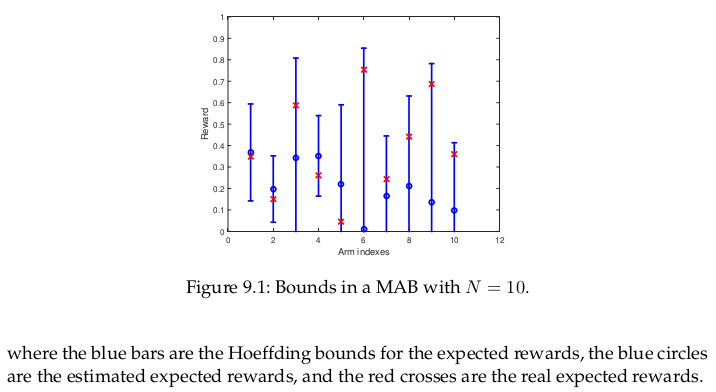
\includegraphics[width=1\textwidth]{images/mab_01.png}
    \end{center}
    \fbox{\begin{minipage}{\linewidth}
        \begin{enumerate}
            \item Which arm would a UCB1 algorithm choose for the next round? Arm 6, which has reward of zero and high bound
            \item Do you think that the figure might be the results obtained by running UCB1 for several rounds? No, UCB1 at each time is trying to keep all upper confidence bound at the same level, but here some arms pulled more times even though others should have been pulled before
            \item Which arm will UCB1 converge to if $T\rightarrow\infty$? Arm 6, since it is the one with highest expected value
            \item Which arm is the one which we pulled the most so far? Arms 2 and 4 as they have the smallest confidence bounds (which are inversely proportional to the number of pulls)
        \end{enumerate}
    \end{minipage}}
    